\documentclass[3p,times]{elsarticle}
\usepackage[utf8]{inputenc}

\usepackage{amssymb,amsmath,latexsym}
\usepackage{soul,color}
\usepackage{xcolor}
\usepackage{graphicx,amssymb}
\usepackage{algorithm}
\usepackage[noend]{algpseudocode}
\usepackage{pgfplots}
\usepackage{array}
\newcolumntype{P}[1]{>{\centering\arraybackslash}p{#1}}
\usepackage{tikz}
\usepackage{caption}
\setcounter{secnumdepth}{4}
\usepackage{hyperref}
\usepackage{float}
\usepackage{subcaption}
\pgfplotsset{compat=newest}
%\usepackage{authblk}
\usepackage{multirow}

\usepackage[outdir=./]{epstopdf}
\usepackage{dblfloatfix}
\usepackage[figuresright]{rotating}

%\pagecolor[rgb]{0.25,0.25,0.25} %black
%\color[rgb]{0.9,0.9,0.9} %grey

\usepackage{ecrc}

\makeatletter %% <- make @ usable in command sequences
\newcount\SOUL@minus
\makeatother  %% <- revert @

%% The ecrc package defines commands needed for running heads and logos.
%% For running heads, you can set the journal name, the volume, the starting page and the authors

%% set the volume if you know. Otherwise `00'
\volume{00}

%% set the starting page if not 1
\firstpage{1}

\setlength{\textfloatsep}{5pt}
%% Give the name of the journal
\journalname{Computer Speech and Language}

%% Give the author list to appear in the running head
%% Example \runauth{C.V. Radhakrishnan et al.}
\runauth{Anidjar et al.}

%% The choice of journal logo is determined by the \jid and \jnltitlelogo commands.
%% A user-supplied logo with the name <\jid>logo.pdf will be inserted if present.
%% e.g. if \jid{yspmi} the system will look for a file yspmilogo.pdf
%% Otherwise the content of \jnltitlelogo will be set between horizontal lines as a default logo

%% Give the abbreviation of the Journal.
\jid{procs}

%% Give a short journal name for the dummy logo (if needed)
\jnltitlelogo{Speech Recognition}

%% Hereafter the template follows `elsarticle'.
%% For more details see the existing template files elsarticle-template-harv.tex and elsarticle-template-num.tex.

%% Elsevier CRC generally uses a numbered reference style
%% For this, the conventions of elsarticle-template-num.tex should be followed (included below)
%% If using BibTeX, use the style file elsarticle-num.bst

%% End of ecrc-specific commands
%%%%%%%%%%%%%%%%%%%%%%%%%%%%%%%%%%%%%%%%%%%%%%%%%%%%%%%%%%%%%%%%%%%%%%%%%%

\newcommand\MyBox[2]{
  \fbox{\lower0.75cm
    \vbox to 1.7cm{\vfil
      \hbox to 1.7cm{\hfil\parbox{1.4cm}{#1\\#2}\hfil}
      \vfil}%
  }%
}

\begin{document}

\begin{frontmatter}

\title{Vision-Based Automatic Landing of Drones}

\author[a,b,c,d]{Or Haim Anidjar\corref{cor1}}
\ead{orhaim@ariel.ac.il}

\author[a]{Moria Grohar}
\ead{moriagro@gmail.com}

\author[a]{Shirel Turgeman}
\ead{shirel.zz10@gmail.com}

% \author[a]{Adi Peisach}
% \ead{adi.peisach@gmail.com}

\author[a, b, c]{Boaz Ben-Moshe}
\ead{benmo@ariel.ac.il}


\address[a]{School of Computer Science, Ariel University, Golan Heights 1, 4077625, Ariel, Israel.}

\address[b]{Ariel Cyber Innovation Center, Ariel University, Golan Heights 1, 4077625, Ariel, Israel.}

\address[c]{Kinematics and Computational Geometry Lab (K\&CG), Ariel University, Golan Heights 1, 4077625, Ariel, Israel.}

\address[d]{Data Science and Artificial Intelligence Research Center, Ariel University, Golan Heights 1, 4077625, Ariel, Israel.}

\cortext[cor1]{Corresponding author: Or Haim Anidjar, School of Computer Science, Ariel University, Golan Heights 1, 4077625, Ariel, Israel.}


\begin{abstract}
This article introduces a platform designed to enable precise landings on the edge of rooftops, facilitating operations at boundary locations. The platform integrates voice recognition capabilities for activation, eliminating reliance on manual button controls. The primary objective is to develop a methodology and control algorithm that allows drones to guard settlements effectively. This research employs a combination of straight-line detection and object detection, avoiding the use of global positioning systems. The system is engineered to operate with drones equipped with existing cameras, obviating the need for additional sensors, and is implemented using the DJI SDK on Android devices. This paper presents a visual landing technology through a proposed algorithm, which is divided into two key tasks: scene evaluation and landing site security. Initially, the drone utilizes object detection to identify and avoid obstacles within the landing area, enabling autonomous descent planning. Once obstacles are cleared, the drone transitions to descent mode. For precise landings at the edge of a rooftop, an edge detection algorithm is employed alongside a target line selection process, allowing the user to designate a specific landing line beforehand, ensuring accuracy during the final approach.
\end{abstract}

\begin{keyword}
Visual-Based Landing \sep Autonomous Landing \sep Accurate Landing\sep Spoken Language Recognition.
\end{keyword}

\end{frontmatter}

\section{Introduction}
Unmanned aerial vehicles (UAVs), commonly known as drones, are aircraft that operate without an onboard pilot, controlled either through radio remote systems or autonomous onboard programs. Drones are valued for their simple yet effective design, ease of operation, flexibility, and cost-efficiency, making them versatile tools in both military and civilian domains. In military operations, they play crucial roles in tasks such as tactical reconnaissance, territorial surveillance, and target acquisition. On the civilian side, drones are utilized for activities like environmental monitoring, weather data collection, and infrastructure inspection. As drones become increasingly prevalent in both sectors, ensuring their safe operation—particularly during landing—has emerged as a critical concern.\\Autonomous drone operations have rapidly advanced, yet precision landing remains a significant challenge, especially in environments where GPS signals are unreliable or unavailable. GPS signals can be easily disrupted by various factors: (a) weather conditions and sunspots may weaken signals, although they typically do not hinder positioning; (b) electromagnetic interference from sources like radios and strong magnetic fields can cause varying degrees of disruption; (c) signal strength diminishes under shelters such as buildings, vehicles, insulation materials, trees, and metal components; and (d) high-rise buildings and dense urban areas can severely impact GPS signal quality. Traditional drone landing methods often rely on GPS, which proves inadequate in urban or indoor settings. This limitation poses significant challenges for applications requiring precise landings, such as urban package delivery, infrastructure inspection, and emergency response. As a result, there is a critical need to develop autonomous positioning and flight control systems for drones that do not rely on GPS signals.\\
This research addresses these challenges by developing a visual-based landing system that enhances accuracy and safety. Our approach enables drones to autonomously identify and land on planar surfaces, such as rooftops, relying solely on visual data from the onboard camera. By eliminating the need for additional sensors or external data inputs, this system offers a robust solution for autonomous landings in complex environments.

\subsection{Authors Contribution}
We propose a visual processing framework that enables the drone to autonomously land by utilizing object (obstacle) detection and edge detection. Our approach is tested on a DJI drone equipped with a standard camera, using the DJI SDK for implementation on Android devices. Additionally, we have implemented a "guard" mode in the app — a button that, when activated, is designed to detect movement (such as people, cars, etc.) and send alerts. The system's robustness is further enhanced by incorporating basic voice commands through a speech recognition module, meeting the requirements outlined by MAFAT.\\

\newpage \section{Algorithm Design} \label{sec:algorithm}
Our proposed algorithm for autonomous drone landing consists of three key components: Target Line Selection, Flight Control, and Object Detection. Each part contributes to the overall reliability and precision of the landing process, ensuring safe navigation and obstacle avoidance.

\begin{figure}[H]
    \centering
    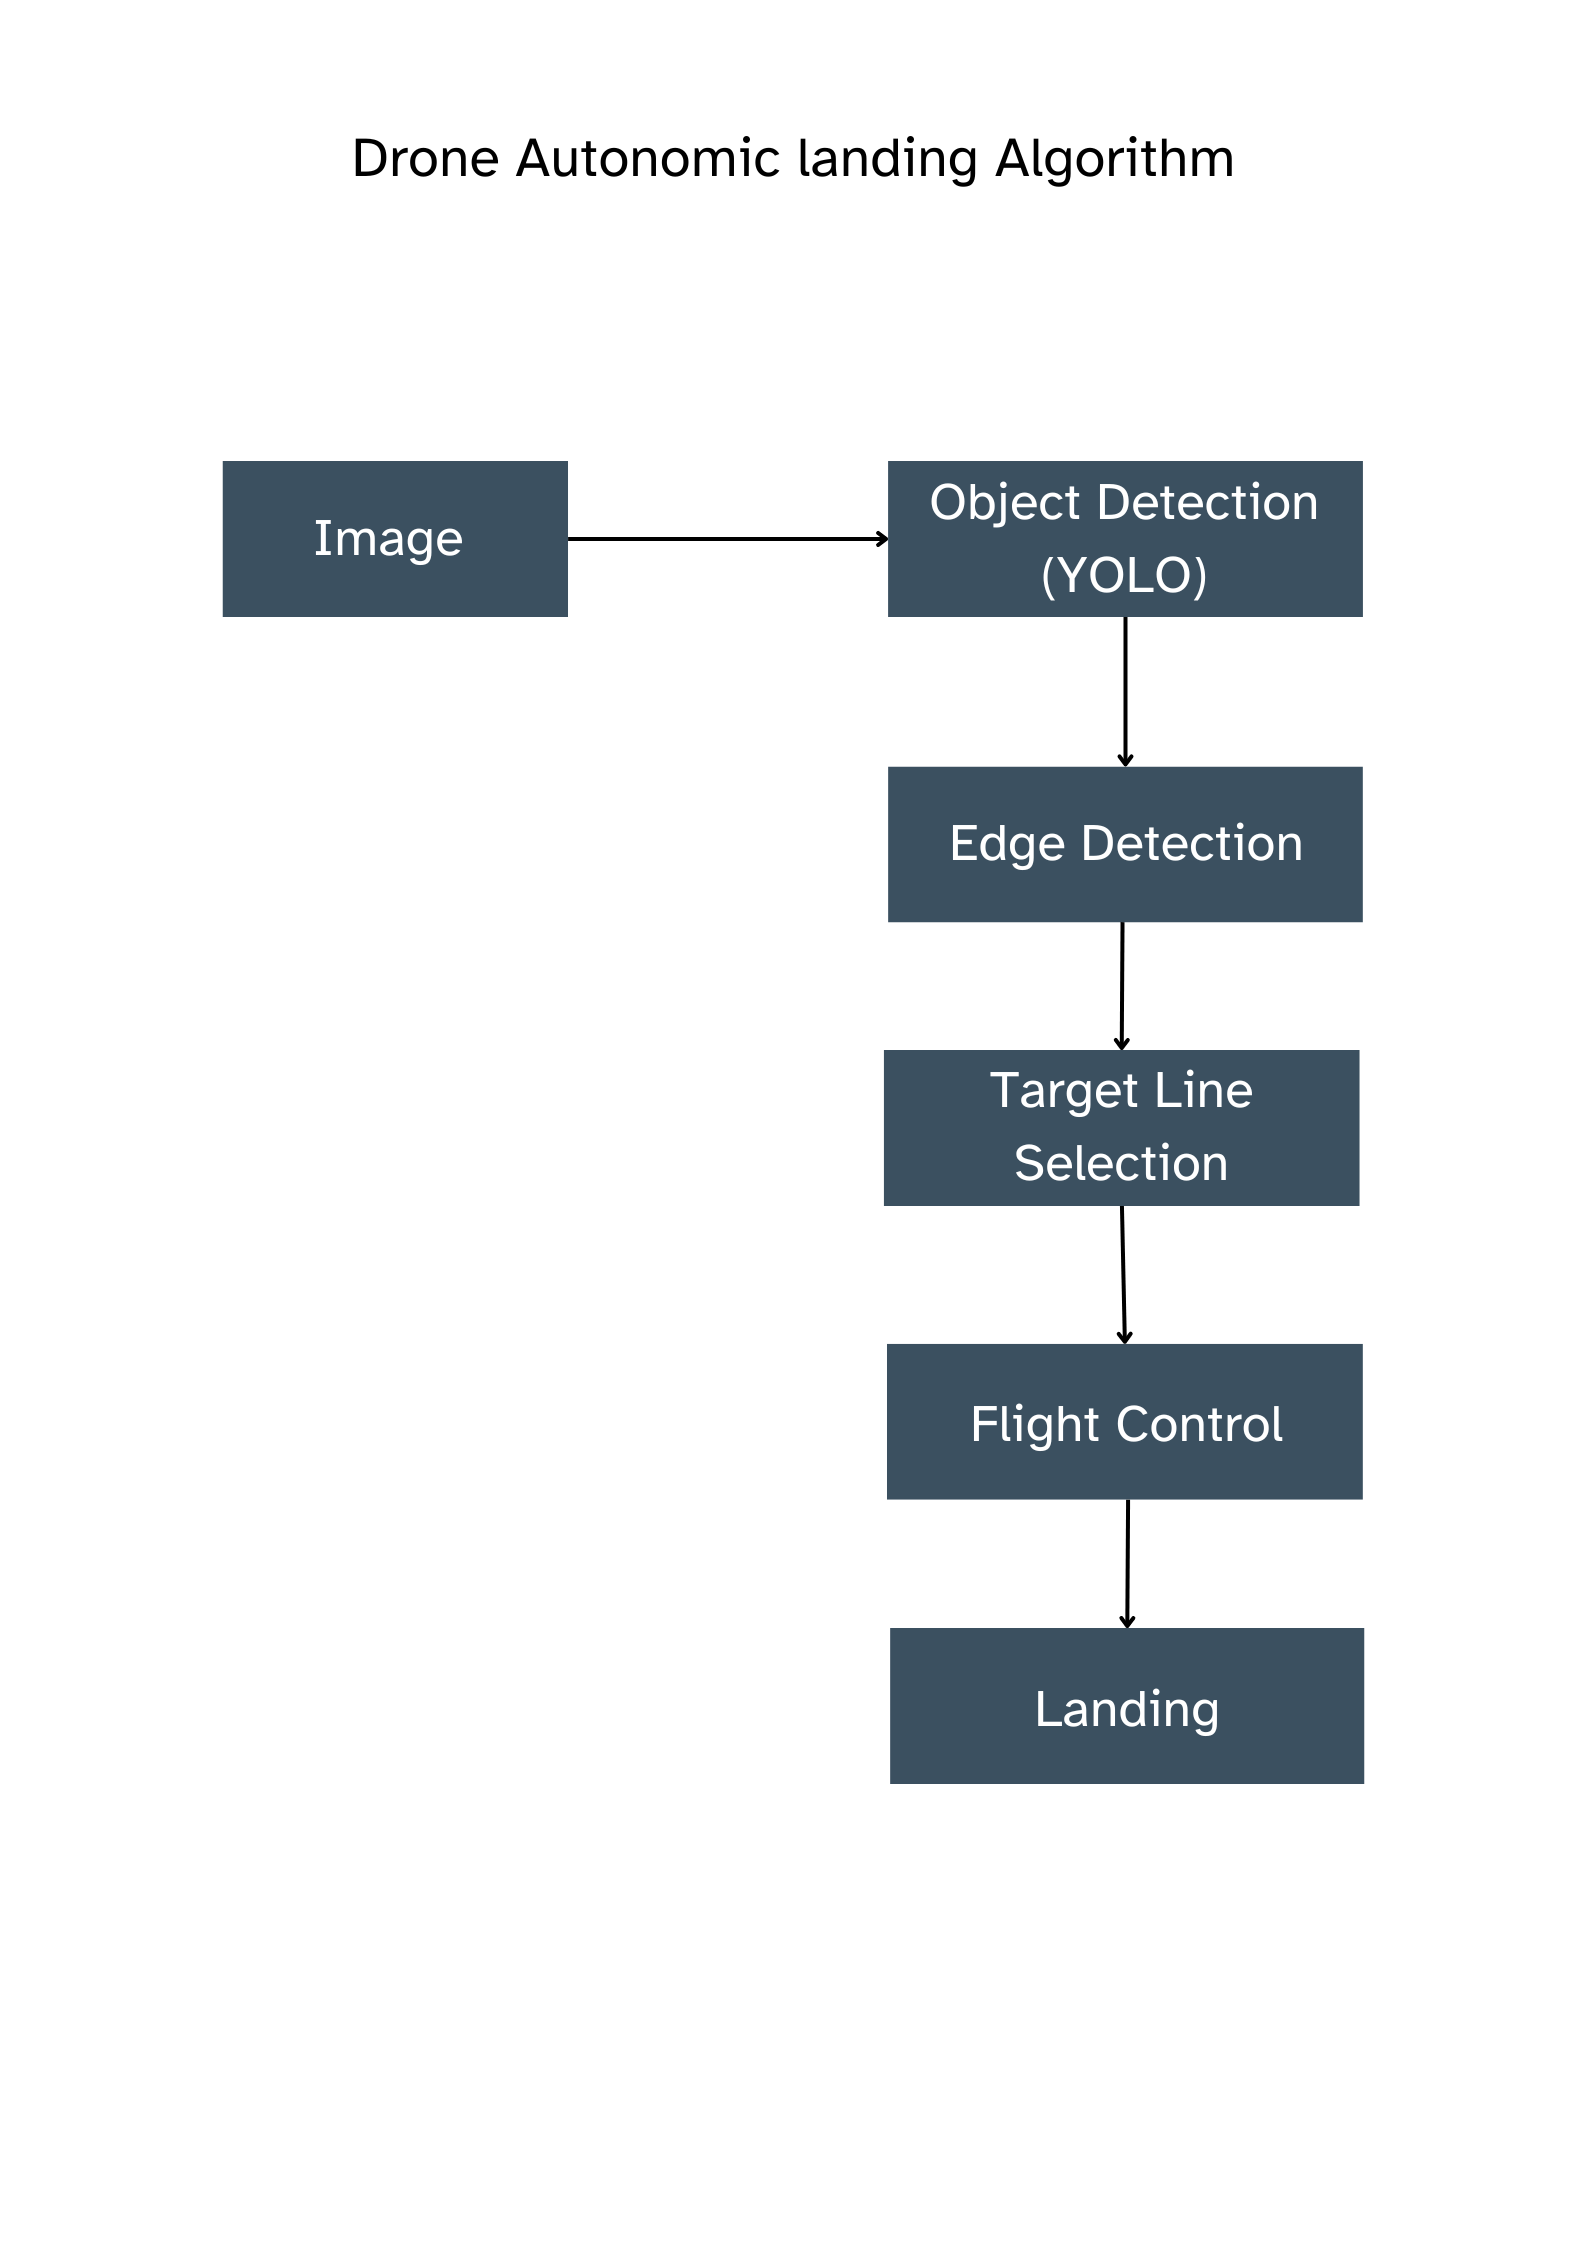
\includegraphics[width=0.7\textwidth]{Schematic_for_automatic_landing.png}  % Reduced the size here
    \caption{Schematic for automatic landing.}
    \label{fig:Schematic_for_automatic_landing.}
\end{figure}

\subsection{Target Line Selection}
In the first stage of the landing process, edge detection is activated to identify all available and compatible lines within the camera's field of view. These lines represent potential landing paths. The user interacts with the system by selecting the desired line for the drone to land behind via a touch-based interface. Once the target line is chosen, the algorithm continuously tracks the line. This is achieved by calculating the distance between the selected line and all detected lines, and the one with the minimum distance is updated as the current target line. This real-time tracking ensures that the drone can maintain accurate navigation towards the desired landing area.

\subsection{Flight Control}
After target line selection, the system activates the flight control module. The drone begins moving towards the selected line by issuing pitch commands, which direct forward movement. This continues until the chosen line is nearly out of the drone’s visible range. Through experimental measurements, we identified a blind spot between the drone's final visible position of the line and its actual location in reality. To compensate for this, the algorithm calculates the necessary adjustment and issues a final pitch command, ensuring that the drone reaches the correct position relative to the target line.

\begin{figure}[H]
    \centering
    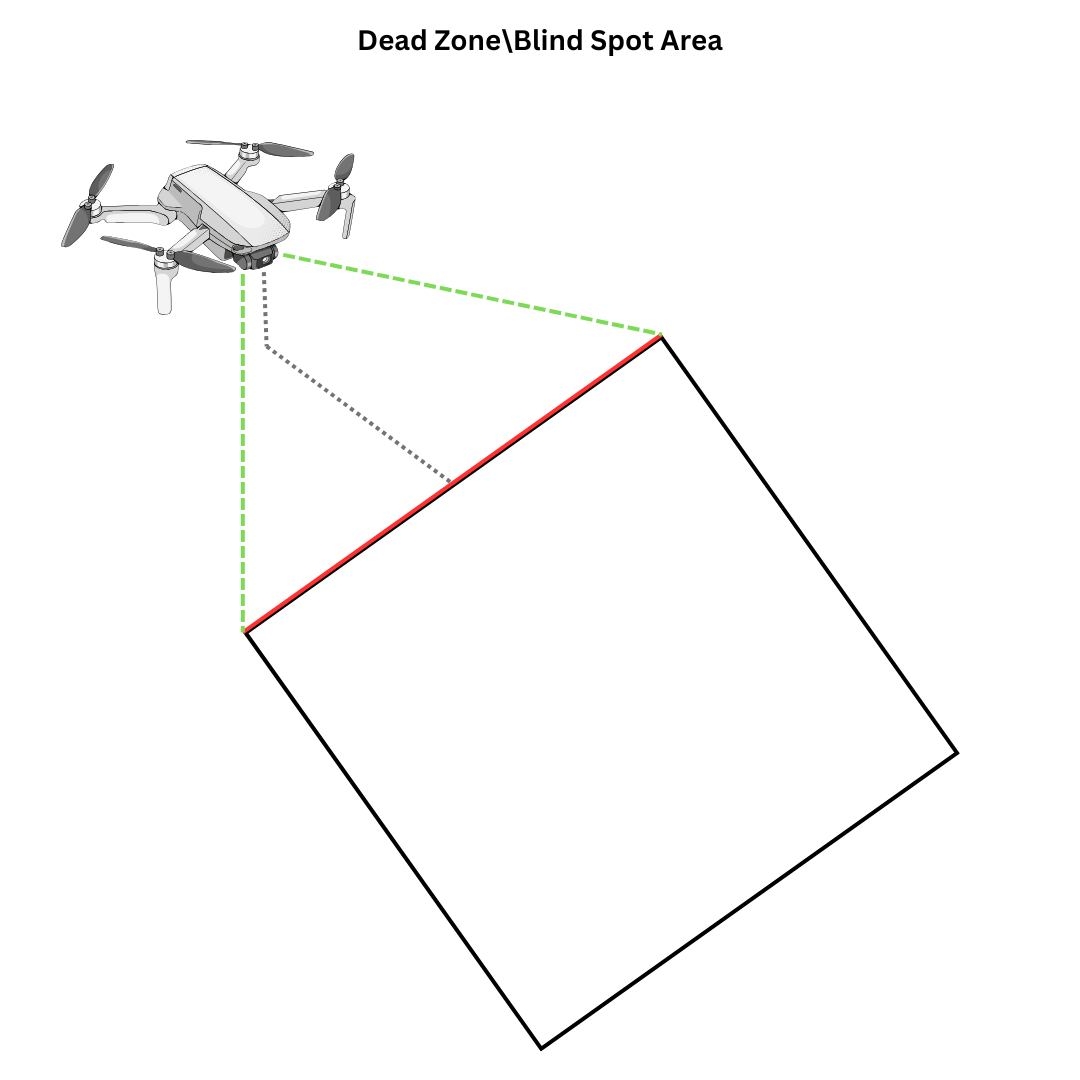
\includegraphics[width=0.7\textwidth]{Blind Spot Area.png}  % Reduced the size here
    % \caption{Schematic for automatic landing.}
    \label{fig:Blind Spot Area.}
\end{figure}

\subsection{Object Detection}
Upon reaching the target area, object detection is initiated to scan for potential hazards in the intended landing zone. The detection algorithm examines the area for obstacles such as people, vehicles, or other objects that may hinder safe landing. The landing zone's dimensions are calculated based on prior measurements from different drone positions, ensuring the detection area is appropriately scaled for accurate hazard identification. If no hazards are detected, the system proceeds with the landing sequence, ensuring a safe and precise touchdown.

\newpage \section{Related Work} \label{sec:related}

\subsection{Obstacle Avoidance}
Obstacle avoidance is a critical aspect of autonomous drone operations, especially in dynamic environments where both static and moving obstacles are present. One approach is integrating depth images with an occupancy voxel map to detect and track dynamic obstacles \cite{xu2023real}. This approach effectively balances computational efficiency with the need for accurate detection and tracking, making it suitable for real-time UAV operations. Another approach involves deep learning techniques like the YOLO (You Only Look Once) framework, which excels at real-time obstacle detection in dynamic environments \cite{redmon2017yolo9000}. YOLO9000 enables rapid detection of multiple objects, making it ideal for fast decision-making in complex surroundings. Its efficiency and accuracy have made it a popular choice for enhancing UAV obstacle avoidance systems.

\subsection{Motion Detection and Object Detection: Yolo (You Only Look Once)}
Recent advancements in motion and object detection have been significantly influenced by the YOLO (You Only Look Once) framework. As highlighted by \cite{dahirou2021motion}, YOLO enables real-time object detection by predicting bounding boxes and class probabilities from full images in a single evaluation, enhancing both speed and accuracy. This capability makes YOLO particularly effective for applications requiring immediate responsiveness, such as surveillance and autonomous navigation.

\subsection{Speech Recognition}
Speech recognition has been explored as a key component in enhancing drone operation through voice commands, particularly in environments where manual control is impractical. Various systems have been developed for continuous speech recognition on Android devices, such as the one proposed by Srivastav et al. \cite{SpeechRecognition}, which enables real-time voice command processing for mobile platforms. This technology is critical for integrating human-drone interaction, especially in hands-free scenarios, allowing operators to issue commands without physical intervention. Such advancements enable drones to act upon voice inputs for tasks like navigation, object detection, or activation of specific modes. Similar systems have been implemented to facilitate the control of unmanned aerial vehicles (UAVs) in real-time, optimizing human-machine interaction and expanding the use cases for drones in dynamic, complex environments.

\subsection{A Robust and Accurate Landing Methodology for Drones on Moving Targets}
Recent work has explored the use of ArUco markers for precision landing in autonomous drones, offering an efficient visual processing solution for target detection and tracking. As demonstrated in \cite{drones6040098}, ArUco markers provide high accuracy in identifying landing zones, especially when combined with robust visual algorithms. This approach addresses common challenges such as variable lighting conditions and drone stability during descent. Implementing these markers has shown success in enhancing landing precision, contributing to safer and more reliable autonomous operations.

\subsection{An improved Canny edge detection algorithm}
Edge detection algorithms play a critical role in enhancing the visual processing capabilities of drones by accurately identifying boundaries and objects within an image. The Canny Edge Detection Algorithm, as discussed in \cite{rong2014improved}, has proven to be highly effective due to its ability to detect edges with minimal noise while maintaining high accuracy. This method ensures that drones can detect and track obstacles, aiding in precise navigation and autonomous landing. Its application in real-time drone systems highlights its importance in improving the robustness of visual navigation and obstacle avoidance.

\section{Drone Control Mechanisms} \label{sec:framework}
The drone’s movement is governed by four fundamental control parameters: yaw, pitch, roll, and throttle. These parameters allow the drone to maneuver in 3D space with precision, facilitating both object tracking and navigation during various flight operations.\\
\begin{description}
\item $\bullet$ Yaw - controls the rotation around the vertical axis, allowing the drone to turn left or right to face objects.
\item $\bullet$ Pitch - adjusts the forward and backward tilt, moving the drone in those directions.
\item $\bullet$ Roll - manages side-to-side tilt, shifting the drone left or right.
\item $\bullet$ Throttle - regulates altitude by increasing or decreasing the drone’s lift.
\end{description}

\section{Framework} \label{sec:framework}
\subsection{Speech Recognition}
The speech recognition system, powered by Google Speech Recognition, continuously listens for the user’s voice until it detects the wake word "hey rexi." Once activated, the system checks subsequent speech for commands from the predefined list, enabling real-time control of the drone without touching the screen. This approach allows the system to remain responsive while minimizing unnecessary processing, facilitating a hands-free operation experience.

Each recognized command triggers a specific action in the drone. The key commands and their associated actions are:
\begin{description}
\item $\bullet$ Takeoff - Initiates the drone's takeoff sequence, lifting it to a designated altitude for hover.
\item $\bullet$ Land - Initiates the landing sequence, lowering the throttle for a controlled descent until the drone reaches the ground.
\item $\bullet$ Stop - Halts any current movement, keeping the drone stationary in hover mode.
\item $\bullet$ Move up - Increases the throttle to elevate the drone vertically.
\item $\bullet$ Move down - Decreases the throttle, causing the drone to descend.
\item $\bullet$ Start recording - Begins video recording using the drone's camera.
\item $\bullet$ Stop recording - Stops the video recording and saves the footage.
\item $\bullet$ Edge detection - Activates the edge detection algorithm, allowing the system to identify and process edges for navigation or object tracking.

\end{description}
\subsection{Object Tracking?}
\subsection{Landing Algorithm}
\subsection{Movement Detection}

\section{Discussion} \label{sec:discussion}

Advancements in language recognition technologies have been noteworthy, yet they confront several challenges and limitations. This discussion highlights some of the prevalent issues:

\begin{enumerate}

    \item \textbf{Linguistic Ambiguity.} Distinguishing between languages with shared linguistic traits

    \item \textbf{Code-Switching Phenomenon.} In multilingual settings,

\end{enumerate}

\newpage \section{Future Work} \label{sec:future}
An important area for future improvement is the algorithm's ability to handle wind conditions, particularly in outdoor environments and at higher altitudes. While the current implementation performs reliably in controlled settings, real-world scenarios—such as fluctuating wind speeds and changing directions—pose significant challenges to the drone's stability and landing accuracy. Specifically, turbulence at great heights can disrupt the drone's trajectory, leading to deviations from the intended flight path and reducing the precision of both target line tracking and landing position.

To address these challenges, we plan to enhance the algorithm by integrating real-time wind compensation techniques. This improvement will involve adapting the flight control module to account for external forces, using sensor and visual data to counteract wind disturbances, and dynamically adjusting the drone's movements. Enhancing wind handling will enable the algorithm to perform more reliably across a wider range of scenarios, ensuring consistent operation in varying environmental conditions.

Additional future work includes transitioning the speech recognition system from an online to an offline model, which will improve reliability by ensuring consistent functionality without internet access. Furthermore, we plan to explore the integration of plane recognition algorithms to enhance landing precision. This capability will enable the drone to autonomously identify suitable landing surfaces, thus increasing safety and operational efficiency.

\section{Conclusion}
In this work, we presented a novel approach for autonomous drone landing using a visual-based framework that eliminates the need for GPS. Our algorithm, tested on a DJI drone equipped with a standard camera, successfully integrates object detection, edge detection, and flight control to enable precise landings. The system's performance in controlled environments demonstrates its effectiveness, especially in scenarios where GPS signals are unreliable or unavailable.\\

However, there are still challenges to address, particularly in handling unpredictable wind conditions and ensuring the system’s reliability in diverse outdoor environments. Future work will focus on improving the algorithm’s robustness in real-world scenarios and enhancing its functionality through additional features such as offline speech recognition and plane recognition algorithms for safer and more autonomous landings.\\

The combination of these developments will pave the way for safer, more reliable, and efficient drone operations in a wide variety of applications, from urban package delivery to military surveillance missions.

% \bibliographystyle{model5-names}\biboptions{authoryear}
% \bibliography{main}
\bibliographystyle{plain}
\bibliography{myDoc}
\end{document}
